% Lezione del 28/04/2021

\documentclass[../main.tex]{subfiles}

\begin{document}
    \section{Istruzioni MIPS}
    Consideriamo una serie di istuzioni MIPS:
    \begin{itemize}
        \item istruzioni di tipo R: \texttt{and}, \texttt{or},
            \texttt{add}, \texttt{sub}, \texttt{slt}
        \item istruzioni della memoria: \texttt{lw}, \texttt{sw}
        \item istruzioni di branch: \texttt{beq}
    \end{itemize}
    \subsection{Gestione del clock}
    L'architettura MIPS è organizzata con la gestione del clock
    in cui vi sono alcune fasi a seconda delle istruzioni eseguite.
    \begin{center}
        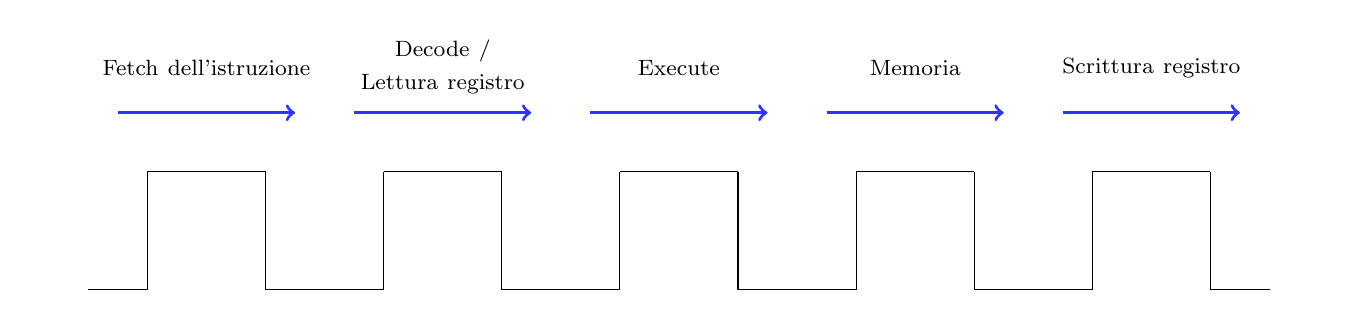
\begin{tikzpicture}[scale=1.5]
            \draw (.5,0) -- (1,0);
            \foreach \x in {0,...,4} {
                \draw (\x * 2 + 1, 0) -- (\x * 2 + 1, 1);
                \draw (\x * 2 + 1, 1) -- (\x * 2 + 2, 1);
                \draw (\x * 2 + 2, 1) -- (\x * 2 + 2, 0);
                \draw (\x * 2 + 2, 0) -- (\x * 2 + 3, 0);
            }
    
            \draw[->, very thick, blue!80] (.75,1.5) -- (2.25,1.5);
            \node[text width=3cm, align=center, text height=2.5mm] at (1.5,1.9) {\footnotesize Fetch dell'istruzione};
    
            \draw[->, very thick, blue!80] (2.75,1.5) -- (4.25,1.5);
            \node[text width=3cm, align=center, text height=2.5mm] at (3.5,1.9) {\footnotesize Decode / \\ Lettura registro};
    
            \draw[->, very thick, blue!80] (4.75,1.5) -- (6.25,1.5);
            \node[text width=3cm, align=center, text height=2.5mm] at (5.5,1.9) {\footnotesize Execute};
    
            \draw[->, very thick, blue!80] (6.75,1.5) -- (8.25,1.5);
            \node[text width=3cm, align=center, text height=2.5mm] at (7.5,1.9) {\footnotesize Memoria};
    
            \draw[->, very thick, blue!80] (8.75,1.5) -- (10.25,1.5);
            \node[text width=3cm, align=center, text height=2.5mm] at (9.5,1.9) {\footnotesize Scrittura registro};

            \draw[white, very thick] (0,0) -- (0.5,0);
            \draw[white, very thick] (10.5,0) -- (11,0);
        \end{tikzpicture}
    \end{center}

    \subsection{Elementi di stato}
    Gli elementi di stato sono i "registri interni" presenti nello schema.
    \\[3mm]
    Tutti gli elementi di stato permettono di fare:
    \begin{itemize}
        \item una \textbf{lettura asincrona}, ovvero non aspettare il colpo
        di clock e rendere il dato disponibile all'uscita del registro
        \item una \textbf{scrittura sincrona}, ovvero per poter aggiornare
        il registro devo attendere il colpo di clock
    \end{itemize}

    \newpage

    \section*{Esempi}
    STEP 1: Leggere l'istruzione dalla memoria \\

    \vspace*{5mm}
    \includegraphics[width=\linewidth]{image/MIPS_architecture}
    \vspace*{5mm}

    \noindent
    STEP 2: Scrivere un'istruzione dentro IR ed aggiornare il PC \\
    In questa fase si conclude la fase di fetch. \\

    \vspace*{5mm}
    \includegraphics[width=\linewidth]{image/MIPS_architecture}
    \vspace*{5mm}

    \noindent
    Osservazioni:
    \begin{itemize}
        \item dando il colpo di clock acquisisco l'istruzione nell'IR
        \item la ALU esegue una \texttt{add} (codice \texttt{010})
        \item con un colpo di clock, l'operazione è disponibile nel momento
        in cui comincia il ciclo con la lettura asincrona e al termine riesco
        a caricare il PC con la scrittura sincrona
        \item in seguito aggiorno il PC
    \end{itemize}

    \vspace*{5mm}

    \noindent
    Lo STEP 1 e 2 sono identici per ogni istruzione.
    Dallo STEP 3 in avanti cambiano le operazioni eseguite.

    \newpage

    \subsection*{Istruzioni della memoria - Esempio \texttt{lw}}
    \texttt{lw rt, offset(rs)}
    \vspace*{1.5mm}

    \begin{adjustwidth}{1cm}{1cm}
        STEP 3a: Leggere \texttt{rs} dal set di registri (istruzione \texttt{ls}) \\

        \begin{figure}[h!]
            \vspace*{5mm}
            \hspace*{1cm} \includegraphics[width=.9\linewidth]{image/MIPS_architecture}
            \vspace*{5mm}
        \end{figure}

        \noindent
        Lettura asincrona del registro \texttt{RD1} attraverso \texttt{A1}.
    \end{adjustwidth}

    \vspace*{3mm}

    \begin{adjustwidth}{1cm}{1cm}
        STEP 3b: Estensione del segno dell'immediato \\

        \begin{figure}[h!]
            \centering

            \vspace*{5mm}
            \hspace*{1cm} \includegraphics[width=.9\linewidth]{image/MIPS_architecture}
            \vspace*{5mm}
        \end{figure}

        \noindent
        Viene fatta l'estensione del segno dell'offset (viene portato
        da 16 a 32 bit).
    \end{adjustwidth}

    \newpage

    \begin{adjustwidth}{1cm}{1cm}
        STEP 4: Calcolare l'indirizzo di memoria \\

        \begin{figure}[h!]
            \centering

            \vspace*{5mm}
            \hspace*{1cm} \includegraphics[width=.9\linewidth]{image/MIPS_architecture}
            \vspace*{5mm}
        \end{figure}

        \noindent
        Bisogna effettuare un'operazione di somma (\texttt{Rs + immediato})
        per ottenere l'indirizzo nel registro del risultato (\texttt{ALUOut}).
    \end{adjustwidth}

    \vspace*{3mm}

    \begin{adjustwidth}{1cm}{1cm}
        STEP 5: Inviare l'indirizzo alla memoria \\

        \begin{figure}[h!]
            \centering

            \vspace*{5mm}
            \hspace*{1cm} \includegraphics[width=.9\linewidth]{image/MIPS_architecture}
            \vspace*{5mm}
        \end{figure}

        \noindent
        Alla fine dell'operazione ho in \texttt{RD}
        la \texttt{word} che dovevo leggere.
    \end{adjustwidth}

    \newpage

    \begin{adjustwidth}{1cm}{1cm}
        STEP 6: Leggere i dati dalla memoria \\

        \begin{figure}[h!]
            \centering

            \vspace*{5mm}
            \hspace*{1cm} \includegraphics[width=.9\linewidth]{image/MIPS_architecture}
            \vspace*{5mm}
        \end{figure}

        \noindent
        Scrivo il valore di \texttt{RD} nel Data Register.
    \end{adjustwidth}

    \vspace*{3mm}

    \begin{adjustwidth}{1cm}{1cm}
        STEP 7: Scrivere il dato nel set dei registri \\

        \begin{figure}[h!]
            \centering

            \vspace*{5mm}
            \hspace*{1cm} \includegraphics[width=.9\linewidth]{image/MIPS_architecture}
            \vspace*{5mm}
        \end{figure}

        \noindent
        Scrivo il valore di \texttt{WD3} nel set dei registri.
    \end{adjustwidth}

    \newpage

    \subsection*{Istruzioni della memoria - Esempio \texttt{sw}}
    \texttt{sw rt, offset(rs)}
    \vspace*{1.5mm}

    \begin{adjustwidth}{1cm}{1cm}
        STEP 3a: Leggere \texttt{rs} e \texttt{rt} dal set dei registri. \\
        
        \begin{figure}[h!]
            \centering

            \vspace*{5mm}
            \hspace*{1cm} \includegraphics[width=\linewidth]{image/MIPS_architecture}
            \vspace*{5mm}
        \end{figure}
    \end{adjustwidth}

    \vspace*{3mm}

    \begin{adjustwidth}{1cm}{1cm}
        STEP 3b: Estensione del segno dell'\texttt{offset} \\
        
        \begin{figure}[h!]
            \centering

            \vspace*{5mm}
            \hspace*{1cm} \includegraphics[width=\linewidth]{image/MIPS_architecture}
            \vspace*{5mm}
        \end{figure}
    \end{adjustwidth}

    \newpage

    \begin{adjustwidth}{1cm}{1cm}
        STEP 4: Calcolare l'indirizzo di memoria \\
        
        \begin{figure}[h!]
            \centering

            \vspace*{5mm}
            \hspace*{1cm} \includegraphics[width=\linewidth]{image/MIPS_architecture}
            \vspace*{5mm}
        \end{figure}

        \noindent
        Molto simile all'esempio della \texttt{lw}. \\
    \end{adjustwidth}

    \vspace*{3mm}

    \begin{adjustwidth}{1cm}{1cm}
        STEP 5a: Inviare l'indirizzo alla memoria \\
        
        \begin{figure}[h!]
            \centering

            \vspace*{5mm}
            \hspace*{1cm} \includegraphics[width=\linewidth]{image/MIPS_architecture}
            \vspace*{5mm}
        \end{figure}
    \end{adjustwidth}

    \newpage

    \begin{adjustwidth}{1cm}{1cm}
        STEP 5b: Inviare il dato alla memoria e attivare
        l'operazione di scrittura \\
        
        \begin{figure}[h!]
            \centering

            \vspace*{5mm}
            \hspace*{1cm} \includegraphics[width=\linewidth]{image/MIPS_architecture}
            \vspace*{5mm}
        \end{figure}
    \end{adjustwidth}

    \newpage

    \subsection*{Istruzioni di tipo R - Esempio \texttt{add}}
    \texttt{add rd, rs, rt}
    \vspace*{1.5mm}

    \begin{adjustwidth}{1cm}{1cm}
        STEP 3: Leggere gli operandi sorgente dal set dei registri e \\
        \hspace*{1.35cm} Scrivere gli operandi sorgente
        nei registri A e B \\
        (TODO: unire l'immagine 3a con la 3b) \\

        \begin{figure}[h!]
            \centering

            \vspace*{5mm}
            \hspace*{1cm} \includegraphics[width=\linewidth]{image/MIPS_architecture}
            \vspace*{5mm}
        \end{figure}
    \end{adjustwidth}

    \begin{adjustwidth}{1cm}{1cm}
        STEP 4: Eseguire l'operazione ALU richiesta

        \begin{figure}[h!]
            \centering

            \vspace*{5mm}
            \hspace*{1cm} \includegraphics[width=\linewidth]{image/MIPS_architecture}
            \vspace*{5mm}
        \end{figure}

        \noindent
        L'etichetta \texttt{XXX} si riferisce ad un valore generico
        (non è un don't care)
    \end{adjustwidth}

    \newpage

    \begin{adjustwidth}{1cm}{1cm}
        STEP 5: Inviare il risultato al set dei registri (\texttt{Rd}) \\

        \begin{figure}[h!]
            \centering

            \vspace*{5mm}
            \hspace*{1cm} \includegraphics[width=\linewidth]{image/MIPS_architecture}
            \vspace*{5mm}
        \end{figure}
    \end{adjustwidth}

    \newpage

\end{document}